\section{Durchführung}

\subsection{Elektronenstrahl im elektrischen Feld}

In diesem Versuch wird zunächst die Proportionalität zwischen $D$ und $U_d$
überprüft bei fünf verschiedenen Beschleunigungsspannungen. Dabei wird die Schaltung
verwendet die in Abbildung \ref{abb:3} dargestellt ist.

\begin{figure}[H]
  \centering
  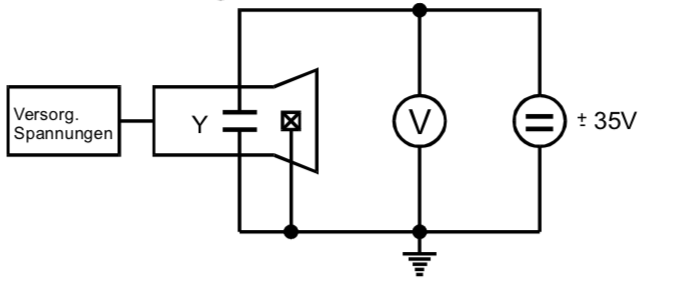
\includegraphics[width=\textwidth]{content/Schaltung1.png}
  \caption{Schaltung zur Bestimmung der Proportionalität von $D$ und $U_d$ \cite{1}.}
  \label{abb:3}
\end{figure}

Daraufhin wird durch Anschließen einer Sägezahnspannung und einer Sinusspannung an
der Kathodenstrahlröhre ein Oszillograph hergestellt. Durch Variation der Sägezahnfrequenz
werden vier verschiedene Frequenzen bestimmt, bei denen ein stehendes Bild der Sinusspannung
zu sehen ist, bei denen also Gleichung \ref{eq:2} erfüllt ist. Dabei wird die Schaltung, die in
Abbildung \ref{abb:4} gezeigt ist verwendet.

\begin{figure}[H]
  \centering
  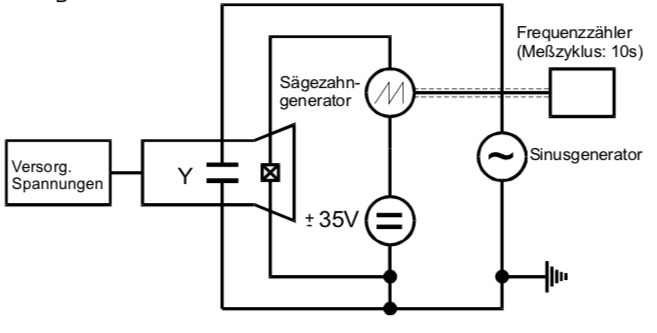
\includegraphics[width=\textwidth]{content/Schaltung2.png}
  \caption{Schaltung für einen Kathodenstrahl-Oszillographen \cite{1}.}
  \label{abb:4}
\end{figure}

\subsection{Elektronenstrahl im transversalen Magnetfeld}

Bei diesem Versuch wird zunächst die Ablenkung von Elektronen durch ein nahezu homogenes
Magnetfeld bestimmt. Dazu wird eine Helmholtz-Spule verwendet. Das Magnetfeld dieser
Spule lässt sich mit folgender Gleichung bestimmen

\begin{equation}
  B = \mu_0 \frac{8 N I}{\sqrt{125} R}.
  \label{eq:4}
\end{equation}

Dabei ist $N$ die Windungszahl, $I$ der Spulenstrom, $R$ der Spulenradius und
$\mu_0$ ist die magnetische Feldkonstante.

Nun wird die Strahlenverschiebung $D$ in Abhängigkeit von dem Magnetfeld $B$ für verschiedene
Beschleunigungsspannungen gemessen.

Daraufhin wird noch das lokale Erdmagnetfeld bestimmt. Dazu wird die Kathodenstrahlröhre
in Nord-Süd-Richtung ausgerichtet. Daraufhin wird die Röhre in Ost-West-Richtung gedreht.
Danach wird das Magnetfeld der Helmholtz-Spule eingeschaltet und so hoch gedreht, dass
die Strahlenverschiebung durch das Erdmagnetfeld kompensiert wird. Dieses Magnetfeld ist dann
die Horizontalkomponente des Magnetfeldes $B_\text{hor}$.
Zur Bestimmung von $B_\text{total}$ wird nun noch der Inklinationswinkel $\varphi$
bestimmt, der Winkel zwischen Horizontalebene und Richtung des Erdfeldes. Dazu wird
ein Kompass in der horizontalen Ebene der Kathodenstrahlröhre in Nord-Süd-Richtung ausgerichtet
und dann um $90°$ geschwenkt. Dann zeigt der Kompass genau $\varphi$ an.


In der Abbildung \ref{abb:5} sind die Abmessungen der Kathodenstrahlröhre dargestellt.

\begin{figure}[H]
  \centering
  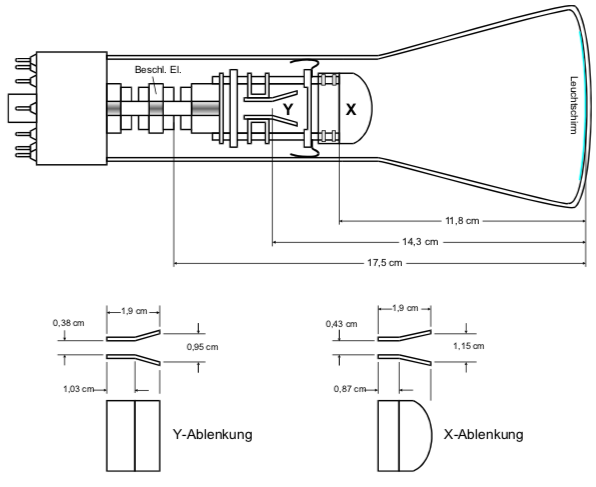
\includegraphics[width=\textwidth]{content/Roehre.png}
  \caption{Konstruktionszeichnung der Kathodenstrahlröhre \cite{1}.}
  \label{abb:5}
\end{figure}
